\documentclass{book}
\usepackage{glossaries}
\usepackage{derivative}
\usepackage{geometry}
\usepackage{pgfplots}
\usepackage{graphicx}
\usepackage{tikz}
\usepackage{float}
\usepackage{lipsum}
\usepackage{minted}
\usepackage{amsmath}
\usepackage{amssymb}
\usetikzlibrary{decorations.pathreplacing,calc}
\geometry{
    left=10mm,
    right=10mm,
    top=10mm,
    bottom=10mm
}
\begin{document}
    \title{
            Queensland University of Technology\\
            \rule{\linewidth}{0.5pt}
        \centering
        \textbf{CAB403} \\
        Systems Programming\\
        \vspace{0.4cm}
        \rule{\linewidth}{1.5pt}
        \small{\textit{Professor Timothy Chappell}}
    }
    \author{Dinal Atapattu}
    \date{\today}
    \maketitle
    \tableofcontents
    \chapter{Introduction to Operating Systems}
        \section{Operating System Structures}
            \subsection{Operating System Services}
                \begin{itemize}
                    \item Operating systems provide an environment for execution of programs and services to programs
                    and users
                    \item Operating System services provides functions that are helpful to the user
                        \begin{itemize}
                            \item User Interface - Almost all opeating systems have a user interface (UI)
                            \begin{itemize}
                                \item Graphical (GUI)
                                \item Command Line (CLI)
                                \item Batch
                            \end{itemize}
                            \item Program Execution - The system must be able to load a program into memory and run that
                            program, end execution, either normally or abnormally (indicating error)
                            \item I/O operations - A running program may require I/O, which involves either a file or I/O device
                        \end{itemize}
                \end{itemize}
    \chapter{Operating System Structures}
    \chapter{Processes}
    \chapter{Threads}
            A thread is a fundamental unit of CPU utilization, which forms the basis of multithreaded computer systems.
            Many modern applications are multithreaded, with threads running within an application. An application can divide tasks to seperate threads
            such as
            \begin{itemize}
                \item Updating the display
                \item Fetching data
                \item Spell checking
                \item Answering network requests
            \end{itemize}
            Thread creation, as opposed to process creation is lightweight, can simplify code, and increase efficiency. For this reason, kernels are often
            multithreaded.
            \begin{figure}[H]
                \centering
                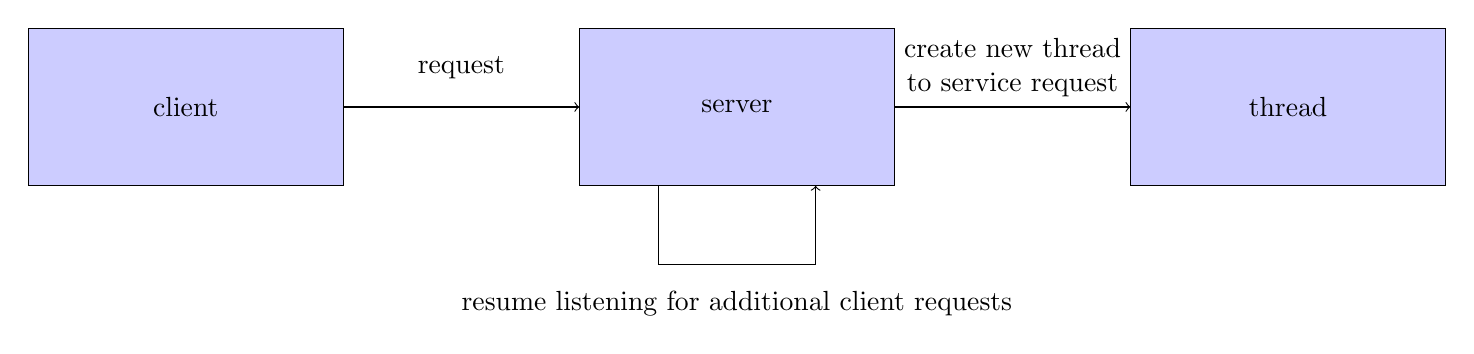
\begin{tikzpicture}
                    \draw [fill=blue!20] (0,0) rectangle (4,2);
                    \draw [->] (4,1) -- (7,1);
                    \draw [fill=blue!20] (7,0) rectangle (11, 2);
                    \draw [->] (11,1) -- (14,1);
                    \draw [fill=blue!20] (14,0) rectangle (18, 2);
                    \draw [->] (8,0) -- (8,-1) -- (10,-1) -- (10,0);
                    \node [align=center] at (2,1) {client};
                    \node [align=center] at (9,1) {server};
                    \node [align=center] at (16,1) {thread};
                    \node [align=center] at (5.5, 1.5) {request};
                    \node [align=center] at (12.5, 1.5) {create new thread\\to service request};
                    \node [align=center] at (9, -1.5) {resume listening for additional client requests};
                \end{tikzpicture}
                \caption{Multithreaded Server Architecture}
            \end{figure}
            Multithreading has the following benefits
            \begin{itemize}
                \item \textbf{Responsiveness}
                    \subitem May allow continued execution if part of a process is blocked, important with user interfaces.
                \item \textbf{Resource Sharing}
                    \subitem Threads share resources of process, easier to manage than shared memory or message parsing.
                \item \textbf{Economy}
                    \subitem Cheaper than process creation, thread switching has lower overhead than context switching.
                \item \textbf{Scalability}
                    \subitem Processes can take advantage of a multiprocessor architecture
            \end{itemize}
        \section{Multicore Programming}
            In the early history of computer design, in order to combat the need for increased computing performance, single-CPU systems
            evoled into mult-CPU systems. Later, this evolved into including multiple compute cores on a single processing chip, where each core
            appears as a seperate CPU to the operating systems. These systems are defined as \textbf{multicore}.
            \subsection{Programming Challenges}
                The trend towards multicore systems continually places pressure on system designers and programmers to make better use of
                multiple compute cores. Designers of operating systems must write scheduling algorithms that use multiple processing cores
                to allow parallel execution
                \begin{figure}[H]
                    \centering
                    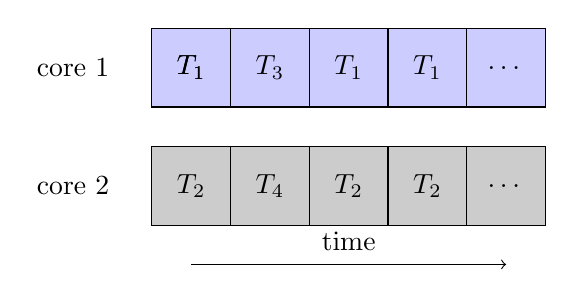
\begin{tikzpicture}
                        \foreach \x in {1,...,5}
                        {    
                            \draw [fill=blue!20] (\x,1.5) rectangle (\x+1,2.5);
                            \draw [fill=black!20] (\x,0) rectangle (\x+1,1);
                        }
                        \draw [->] (1.5,-0.5) -- (5.5,-0.5);
                        \node [align=center] at (3.5, -0.2) {time};
                        \node [align=center] at (0, 2) {core 1};
                        \node [align=center] at (0, 0.5) {core 2};
                        \node [align=center] at (1.5, 2) {$T_1$};
                        \node [align=center] at (1.5, 0.5) {$T_2$};
                        \node [align=center] at (2.5, 2) {$T_3$};
                        \node [align=center] at (2.5, 0.5) {$T_4$};                        \node [align=center] at (1.5, 2) {$T_1$};
                        \node [align=center] at (3.5, 2) {$T_1$};
                        \node [align=center] at (3.5, 0.5) {$T_2$};  
                        \node [align=center] at (4.5, 2) {$T_1$};
                        \node [align=center] at (4.5, 0.5) {$T_2$};
                        \node [align=center] at (5.5, 2) {$\dots$};
                        \node [align=center] at (5.5, 0.5) {$\dots$};  
                    \end{tikzpicture}
                    \caption{Parallel Execution on a Multicore System}
                \end{figure}
            In general, five areas present challenges in programming for multicore systems
            \begin{itemize}
                \item Identifying tasks
                    \subitem This involves examining applications to find areas that can be divided into seperate, concurrent tasks. Ideally, tasks
                    are independent of one another and thus can run in parallel on individual cores
                \item Balance
                    \subitem While Identifying tasks that run in parallel, programmers msut also ensure that tasks perform equal work of equal value.
                    In some instances, a certain task may not contribute as much value to the overall process as other tasks. Using seperate execution cores
                    for that task might not be worth the cost
                \item Data Splitting
                    \subitem Data accessed and manipulated by tasks must be divded to run on seperate cores, similar to how applications are divided to seperate tasks
                \item Data Dependency
                    \subitem The data accessed by he tasks must be examined for dependencies between the two or more tasks. When data is dependent between cores,
                    programmers must ensure that the execution of the tasks is synchronized to accomodate the dependency.
                    \begin{figure}[H]
                        \centering
                        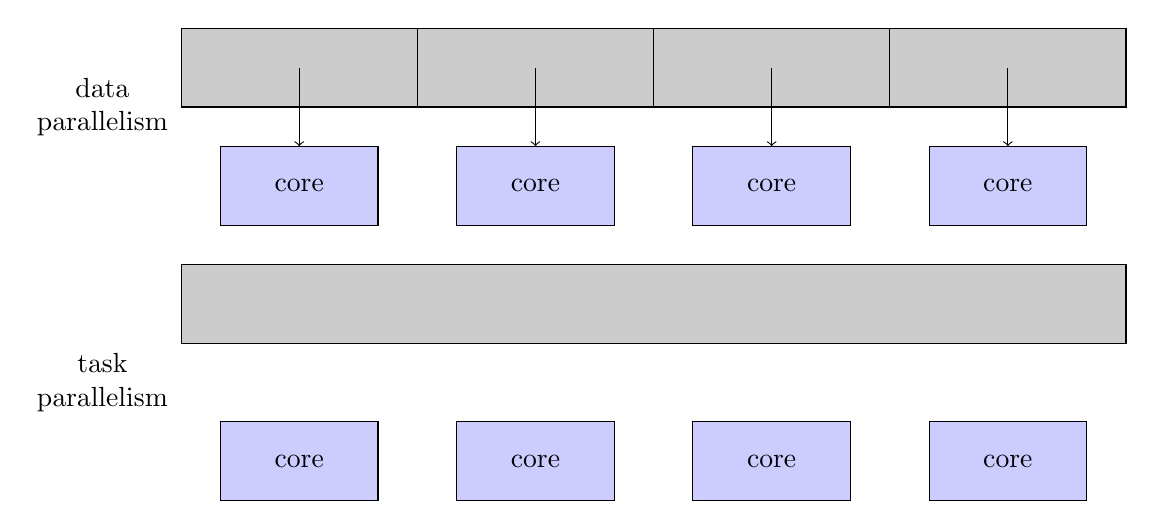
\begin{tikzpicture}
                            \draw [fill=black!20] (0,2) rectangle (12,3);
                            \foreach \x in {0,3,6,9}
                            {
                                \draw [fill=black!20] (\x, 5) rectangle (\x+3,6);
                                \draw [->] (\x+1.5, 5.5) -- (\x+1.5, 4.5);
                                \draw [fill=blue!20] (\x+0.5,3.5) rectangle (\x+2.5,4.5);
                         \draw [fill=blue!20] (\x+0.5,1) rectangle (\x+2.5,0);
                            }
                            \foreach \x in {0.5,...,3.5}
                            {
                                \node at (\x*3, 4) {core};
                                \node at (\x*3, 0.5) {core};
                            }
                            \node [align=center] at (-1, 5) {data\\parallelism};
                            \node [align=center] at (-1, 1.5) {task\\parallelism};
                        \end{tikzpicture}
                        \caption{Data and Task Parallism}
                    \end{figure}
                \item Testing and Debugging
                    \subitem When a program is running in parallel n multiple cores, many different execution paths are possible. Testing and debugging such
                    concurrent programs is inherently more difficult than testing and debugging single threaded applications
            \end{itemize}
            \subsection{Parallelism}
                Types of parallelism
                \begin{itemize}
                    \item Data Parallelism
                        \subitem Focuses on distributing subsets of the same data across multiple compute cores, performing the same operation on each core.
                        \subitem Example: summing the contents of an array size $N$, on a dual core system, thread A sums the elements [0] ... [$N/2 - 1$], thread B
                        sums the elements $[N/2]$ ... $[N-1]$. These threads will run in parallel on seperate cores.
                    \item Task Parallelism
                        \subitem Distributes tasks across multiple cores. Each thread peforms a unique operation. Different threads may operate on the same or different
                        data.
                        \subitem Example: Dual core system, applying two different arithmetic and/or other operation on the same block of data on seperate threads. These
                        threads will will run parallel on seperate cores.
                \end{itemize}
                Data and Task parallelism may be done together, in a hybrid solution.
                \begin{figure}[H]
                    \centering
                    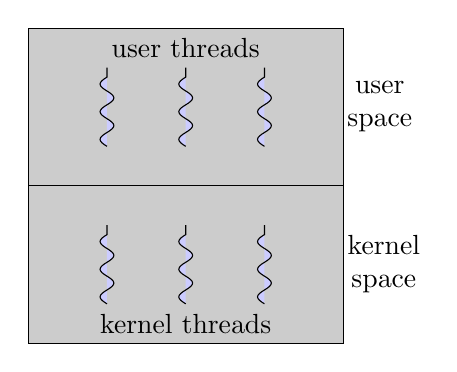
\begin{tikzpicture}
                        \draw [fill=black!20] (0,2) rectangle (4,4);
                        \draw [fill=black!20] (0,0) rectangle (4,2);
                        \foreach \x in {1,...,3}
                        {
                            \draw[fill=blue!20, decorate,decoration={coil,aspect=0}] (\x,0.5) -- (\x,1.5);
                            \draw[fill=blue!20, decorate,decoration={coil,aspect=0}] (\x,2.5) -- (\x,3.5);
                        }
                        \node [below] at (2,4) {user threads};
                        \node [above] at (2,0) {kernel threads};
                        \node [align=center, left] at (5,3) {user\\space};
                        \node [align=center, left] at (5.1,1) {kernel\\space};
                    \end{tikzpicture}
                \end{figure}
        \section{Multithreading Models}
            \subsection{Many-To-One Model}
                Many user-level threads are mapped to a single kernel thread.\\
                One thread block causes all to block.\\
                Multiple threads cannot run in parallel on a multicore system because the kernel can only handle a single thread.\\
                Rarely used.\\
                Examples include
                \begin{itemize}
                    \item Solaris Green threads
                    \item GNU Portable threads
                \end{itemize}
                \begin{figure}[H]
                    \centering
                    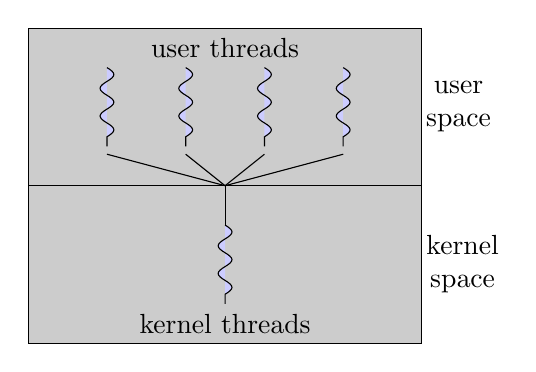
\begin{tikzpicture}
                        \draw [fill=black!20] (0,1) rectangle (5,3);
                        \draw [fill=black!20] (0,3) rectangle (5,5);
                        \foreach \x in {1,...,4}
                        {
                            \draw[fill=blue!20, decorate, decoration={coil,aspect=0}] (\x,4.5) -- (\x,3.5);
                            \draw (\x,3.4) -- (2.5,3);
                        }
                        \draw (2.5, 3) -- (2.5,2.5);
                        \draw[fill=blue!20, decorate, decoration={coil,aspect=0}] (2.5, 2.5) -- (2.5, 1.5);
                        \node [above] at (2.5,4.5) {user threads};
                        \node [above] at (2.5,1) {kernel threads};
                        \node [left, align=center] at (6,4) {user\\space};
                        \node [left, align=center] at (6.1,2) {kernel\\space};
                    \end{tikzpicture}
                    \caption{Many-to-one model}
                \end{figure}
            \subsection{One-To-One Model}
                Each user-level thread maps to a kernel thread.\\
                Creating a user level thread creates a kernel thread.\\
                More concurrency than many-to-one.\\
                Number of threads per process sometimes restricted due to overhead.\\
                Examples include.
                \begin{itemize}
                    \item Windows
                    \item Linux
                    \item Solaris (9 and later)
                \end{itemize}
                \begin{figure}[H]
                    \centering
                    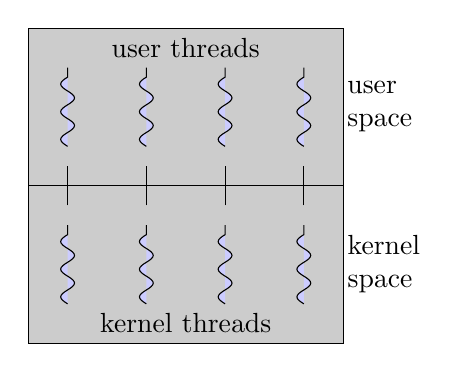
\begin{tikzpicture}
                        \draw [fill=black!20] (0.5,0.5) rectangle (4.5,2.5);
                        \draw [fill=black!20] (0.5,2.5) rectangle (4.5,4.5);
                        \foreach \x in {1,...,4}
                        {
                            \draw[fill=blue!20, decorate, decoration={coil,aspect=0}] (\x,1) -- (\x,2);
                            \draw[fill=blue!20, decorate, decoration={coil,aspect=0}] (\x,3) -- (\x,4);
                            \draw (\x,2.25) -- (\x,2.75);
                        }
                        \node [below, align=center] at (2.5,1) {kernel threads};
                        \node [above, align=center] at (2.5,4) {user threads};
                        \node [left, align=left] at (5.5,3.5) {user\\space};
                        \node [left, align=left] at (5.6,1.5) {kernel\\space};
                    \end{tikzpicture}
                    \caption{One-to-one model} 
                \end{figure}
            \subsection{Many-to-many model}
                Allows many user level threads to be mapped to many kernel threads.\\
                Allows the operating system to create a sufficient number of kernel threads.\\
                Examples include
                \begin{itemize}
                    \item Solaris (pre version 9)
                    \item Windows (\textit{ThreadFiber} package)
                \end{itemize}
                \begin{figure}[H]
                    \centering
                    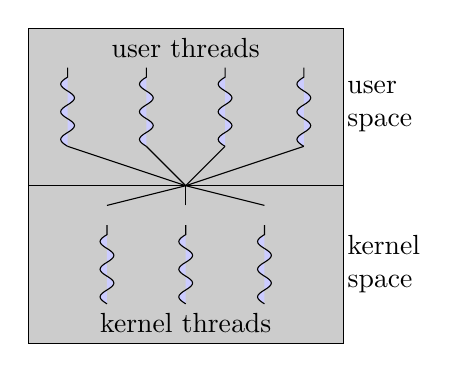
\begin{tikzpicture}
                        \draw [fill=black!20] (0.5,0.5) rectangle (4.5,2.5);
                        \draw [fill=black!20] (0.5,2.5) rectangle (4.5,4.5);
                        \foreach \x in {1,...,4}
                        {
                            \draw[fill=blue!20, decorate, decoration={coil,aspect=0}] (\x,3) -- (\x,4);
                            \draw (\x,3) -- (2.5,2.5);
                        }
                        \foreach \x in {1.5,...,3.5}
                        {
                            \draw[fill=blue!20, decorate, decoration={coil,aspect=0}] (\x,1) -- (\x,2);
                            \draw (\x,2.25) -- (2.5,2.5);
                        }
                        \node [below, align=center] at (2.5,1) {kernel threads};
                        \node [above, align=center] at (2.5,4) {user threads};
                        \node [left, align=left] at (5.5,3.5) {user\\space};
                        \node [left, align=left] at (5.6,1.5) {kernel\\space};
                    \end{tikzpicture}
                    \caption{Many-to-many model}
                \end{figure}
            \subsection{Two-level model}
                Similar to Many-to-many, except allows a user thread to be \textbf{bound} to a kernel thread
                Examples include
                \begin{itemize}
                    \item IRIX
                    \item HP-UX
                    \item Tru64 UNIX
                    \item Solaris (8 and earlier)
                \end{itemize}
                \begin{figure}[H]
                    \centering
                    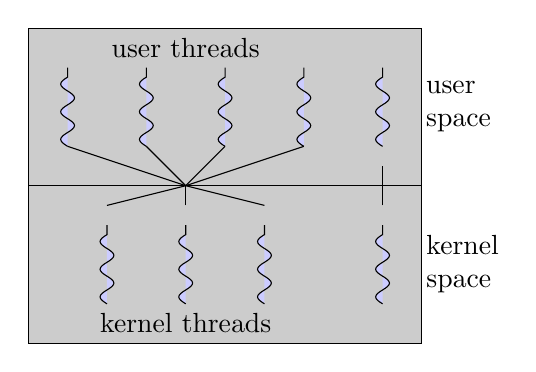
\begin{tikzpicture}
                        \draw [fill=black!20] (0.5,0.5) rectangle (5.5,2.5);
                        \draw [fill=black!20] (0.5,2.5) rectangle (5.5,4.5);
                        \foreach \x in {1,...,4}
                        {
                            \draw[fill=blue!20, decorate, decoration={coil,aspect=0}] (\x,3) -- (\x,4);
                            \draw (\x,3) -- (2.5,2.5);
                        }
                        \foreach \x in {1.5,...,3.5}
                        {
                            \draw[fill=blue!20, decorate, decoration={coil,aspect=0}] (\x,1) -- (\x,2);
                            \draw (\x,2.25) -- (2.5,2.5);
                        }
                        \draw[fill=blue!20, decorate, decoration={coil,aspect=0}] (5,3) -- (5,4);
                        \draw[fill=blue!20, decorate, decoration={coil,aspect=0}] (5,1) -- (5,2);
                        \draw (5,2.25) -- (5,2.75);
                        \node [below, align=center] at (2.5,1) {kernel threads};
                        \node [above, align=center] at (2.5,4) {user threads};
                        \node [left, align=left] at (6.5,3.5) {user\\space};
                        \node [left, align=left] at (6.6,1.5) {kernel\\space};
                    \end{tikzpicture}
                    \caption{Two-level model}
                \end{figure}
        \section{Thread Libraries}
            \subsection{Pthreads}
                Refers to the POSIX standard (IEEE 1003.1c) defining an API for thread creation and synchronisation.
                This is a specification not an implementation
                \begin{figure}[H]
                    \centering
                    \inputminted{c}{code/threads/pthreads.c}
                    \caption{Multithreading using the pthreads API}
                \end{figure}
                Although Windows does not natively support pthreads, some third-party implementations are available
                \begin{figure}[H]
                    \centering
                    \begin{minted}{c}
                        #define NUM_THREADS 10
                        /* an array of threads to be joined upon */
                        pthread_t workers[NUM_THREADS];

                        for (int i = 0; i < NUM_THREADS; i++)
                        {
                            pthread_join(workers[i], NULL);
                        }
                    \end{minted}
                    \caption{Joining 10 threads using the pthreads API}
                \end{figure}
            \subsection{Windows Threads}
                Similar to the technique used in pthreads. Uses a different library
                \begin{figure}[H]
                    \centering
                    \inputminted{c}{code/threads/windows_threads.c}
                    \caption{Multithreading using the Windows API}
                \end{figure}
        \section{Implicit Threading}
            The growing popularity of multicore processing means that applications now require hundreds,
            or thousands of threads. When designing such programs, correctness grows more and more difficult.
            Creating and management of threads done by compilers and run-time libraries are favoured in this case.
            \subsection{Thread Pools}
                Creates a number of threads in a pool where they await work
                Advantages
                \begin{itemize}
                    \item Usually faster to service a request with an existing thread than create a new thread
                    \item Alows the number of threads in an application(s) to be bound to the size of the pool
                    \item Seperating tasks to be performed from mechanics of creating task allows different stratgeies for
                    running task
                        \subitem Tasks could be scheduled to be run periodically
                \end{itemize}
                \begin{figure}[H]
                    \centering
                    \begin{minted}{c}
                        DWORD WINAPI PoolFunction(PVOID Param)
                        {
                            /*
                            * this function runs as a seperate thread
                            */
                        }
                    \end{minted}
                    \caption{Thread pooling in the Windows API}
                \end{figure}
            \subsection*{OpenMP}
                Set of compiler directives and an API for C, C++, FORTRAN.\\
                Provides support for parallel programming and shared-memory environments.\\
                Identifies \textcolor{blue}{parallel regions} - blocks of code that can run in parallel.\\
                \begin{figure}[H]
                    \centering
                    \inputminted{c}{code/threads/openmp.c}
                    \caption{OpenMP}
                \end{figure}
            \subsection{Grand Central Dispatch}
                \begin{itemize}
                    \item Apple technology for Mac OS X and iOS operating systems
                    \item Extensions to C, C++, API and run-time library
                    \item Allows identification of parallel sections
                    \item Manages most details of threading
                    \item Blocks is in "\textasciicircum\{\}" - \mintinline{c}{^{ printf("I am a block"); }}
                    \item Blocks are placed in dispatch queue and then assigned to avaiable threads in thread pool when removed
                    \item Two types of dispatch queues
                        \begin{itemize}
                            \item \textbf{Serial} - blocks are removed FIFO, queue is per process, called \textbf{Main Queue}
                                \subitem Programmers create additional serial queues within program
                            \item \textbf{Concurrent} - removed in FIFO, but many be removed at a time
                                \subitem Three system wide queues with priorities \textcolor{blue}{low, default, high}
                                \begin{figure}[H]
                                    \begin{flushleft}
                                        \begin{minted}{c}
dispatch_queue_t queue = dispatch_get_global_queue(DISPATCH_QUEUE_PRIORITY_DEFAULT, 0);
dispatch_async(queue, ^{ printf("I am a block."); });
                                        \end{minted}
                                    \end{flushleft}
                                \end{figure}
                        \end{itemize}
                \end{itemize}
        \section{Threading Issues}
            \begin{itemize}
                \item Semantics of \textbf{fork()} and \textbf{exec()} system calls.
                \item Signal handling (synchronous and asynchronous)
                \item Thread cancellation of target thread (asynchronous or deferred)
                \item Thread local storage
                \item Scheduler activations
            \end{itemize}
            \subsection{Semantics of fork() and exec()}
                \begin{itemize}
                    \item Does fork() duplicate only the calling thread or all threads?
                        \subitem Some UNIXes have two versions of fork
                    \item exec() usually works as normal (replaces running process including all threads)
                \end{itemize}
            \subsection{Signal Handling}
                \begin{itemize}
                    \item \textcolor{blue}{Signals} are used in UNIX systems to notify a process that a particular event has occurred
                    \item A \textcolor{blue}{signal handler} is used to process signals
                        \begin{itemize}
                            \item Signal is generated by an event
                            \item Signal is delivered to a process
                            \item Signal is handled by one of two signal handlers
                                \subitem default
                                \subitem user-defined
                        \end{itemize}
                    \item Every signal has a \textcolor{blue}{default handler} that kernel runs when handling a signal
                        \begin{itemize}
                            \item \textcolor{blue}{User-defined signal handler} can override default
                            \item For single-threaded, signal delivered to process
                        \end{itemize}
                    \item Where is the signal delivered in multi-threaded?
                        \begin{itemize}
                            \item Deliver the signal to the thread to which the signal applies
                            \item Deliver the signal to every thread in the process
                            \item Deliver the signal to certain threads in process
                        \end{itemize}
                \end{itemize}
            \subsection{Thread Cancellation}
                \begin{itemize}
                    \item Terminating a thread before it has finished
                    \item Thread to be canceled is \textcolor{blue}{target thread}
                    \item Two general approaches
                        \begin{itemize}
                            \item \textbf{Asynchronous cancellation} terminates the target thread immediately
                            \item \textbf{Deferred cancellation} allows the target thread to periodically check if it should be cancelled
                        \end{itemize}
                        \begin{figure}[H]
                            \begin{minted}{c}
                                pthread_t thread_id;
                                /* create the thread */
                                pthread_create(&thread_id, 0, worker, NULL);
                                ...
                                /* cancel the thread */
                                pthread_cancel(thread_id);
                            \end{minted}
                            \caption{pthread code to create and cancel a thread}
                        \end{figure}
                    \item Invoking thread cancellation requests cancellation, but actual cancellation depends on the thread state
                        \begin{figure}[H]
                            \centering
                            \begin{tabular}{|c|c|c|}
                                \hline
                                \textbf{Mode} & \textbf{State} & \textbf{Type}\\
                                \hline
                                Off & Disabled & -\\
                                \hline
                                Deferred & Enabled & Deferred\\
                                \hline
                                Asynchronous & Enabled & Asynchronous\\
                                \hline
                            \end{tabular}
                            \caption{Thread States}
                        \end{figure}
                    \item If a thread has cancellation disabled, cancellation remains pending till enabled
                    \item Default type is deferred
                        \subitem Cancellation only occurs when thread reaches \textcolor{blue}{cancellation point}
                            \begin{itemize}
                                \item i.e., \mintinline{c}{pthread_testcancel();}
                                \item Then \textcolor{blue}{cleanup handler} is invoked
                            \end{itemize}
                    \item On Linux, thread cancellation is handled through signals
                \end{itemize}
            \subsection{Thread-Local Storage}
                \begin{itemize}
                    \item \textcolor{blue}{Thread-local-storage (TLS)} allows each thread to have its own copy of data
                    \item Useful when you don't have control over thread creation (i.e., using a thread pool)
                    \item Different from local variables
                        \begin{itemize}
                            \item Local variables visible only during single function invocation
                            \item TLS visible across function invocations
                        \end{itemize}
                    \item Similar to static data
                        \begin{itemize}
                            \item TLS is unique to each thread
                        \end{itemize}
                \end{itemize}
            \subsection{Scheduler Activations}
                \begin{itemize}
                    \item Both Many to Many and Two-Level require communication to maintain the appropriate 
                    number of kernel threads allocated to the application
                    \item Typically use an intermediate data structure between user and kernel threads (\textcolor{blue}{lightweight process (LWP)})
                        \begin{itemize}
                            \item Appears to be a virtual processor on which process can schedule user thread to run
                            \item Each LWP is attached to a kernel thread
                            \item How many LWPs to create?
                        \end{itemize}
                    \item Scheduler activations provide \textcolor{blue}{upcalls} - a communication mechanism from the kernel
                    to the \textcolor{blue}{upcall handler} in the thread library
                    \item This communication allows an application to maintain the correct number of kernel threads
                \end{itemize}
                \begin{figure}[H]
                    \centering
                    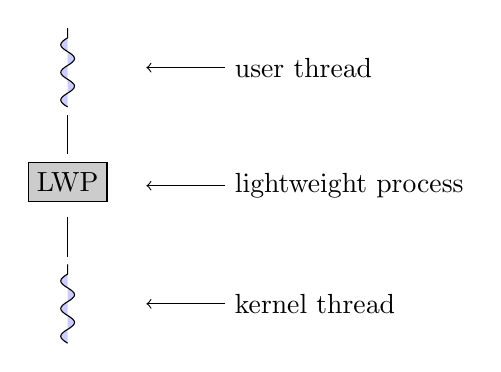
\begin{tikzpicture}
                        \foreach \y in {0,3}
                        {
                            \draw [fill=blue!20, decorate, decoration={coil,aspect=0}] (0,\y) -- (0,\y+1);
                        }
                        \foreach \y in {1.1, 2.4}
                        {
                            \draw (0,\y) -- (0,\y+0.5);
                        }
                        \draw [fill=black!20] (-0.5,1.8) rectangle (0.5,2.3);
                        \node [align=center] at (0,2.05) {LWP};
                        \foreach \y in {0.5,2,3.5}
                        {
                            \draw [->] (2,\y) -- (1,\y);
                        }
                        \node [align=left, right] at (2,0.5) {kernel thread};
                        \node [align=left, right] at (2,2) {lightweight process};
                        \node [align=left, right] at (2,3.5) {user thread};
                    \end{tikzpicture}
                    \caption{Lightweight Process (LWP)}
                \end{figure}
    \chapter{Synchronisation}z
    \chapter{Safety Critical Systems}
        \textbf{Safety} is the freedom from conditions that cause death, injury, illness, damage
        to or loss of equipment or property, or environmental harm\\
        Software is inherently not safe or unsafe, however can contribute to unsafe conditions in a
        safety critical system. Such software is \textbf{Safety Critical}\\
        IEEE definition: "Software whose use in a system can result in unacceptable risk. Safety-critical
        software incliudes softwre whose operation or failure to operate can lead to a hazardous state.
        Software intended to reover from hazardous states, and software intended to mitigate the severity
        of an incident"
        \section{MISRA C}
            \begin{itemize}
                \item Motor Industry Software Reliability Association
            \end{itemize}
        \section{NASA Power of 10}
            \begin{itemize}
                \item Avoid complex flow constructs (\textcolor{red}{goto, recursion, jumps})
                \item All loops must have fixed bounds (prevents runaway code)
                \item Avoid \textcolor{red}{heap memory allocation} (no malloc, define everything in main)
                \item Restrict functions to a single page (max 50 lines)
                \item Use a minimum of \textcolor{red}{two} runtime assertions per function
                \item Restrict the scope of data to the smallest possible
                \item Check the return value of all non-void functions, or cast to void to indicate the return is useless
                \item Use the preprocessor sparingly. (\textcolor{red}{DO NOT USE} stdio.h, local.h, abort/exit/system from stdlib.h, time handling from time.h)
                \item Limit pointer use to a \textcolor{red}{single dereference} and \textcolor{red}{DO NOT USE FUNCTION POINTERS}
                \item Compile with all warnings active (Wall, Wextra, etc.) all warnings should then be addressed before release
            \end{itemize}
    \chapter{Distributed Systems}
        A distributed system is a collection of processors that do not share memory or
        a clock. Instead, each node has its own local memory. The nodes communicate over 
        various networks, such as high-speed busses.\\
        Applications of distributed systems vary widely, from providing transparent file access
        inside an organization, to large-scale cloud storage services, to business analysis of 
        trends on large datasets, to parallel processing of scientific data. With the most 
        ubiqiutous form of a distributed system being the Internet.
        \section{Basic Concepts}
            A \textcolor{blue}{distributed system} is a collection of loosely coupled nodes
            interconnected by a communication network. From the point of view of a specific node
            in a distributed system, the rest of the nodes and their respective resources are remote,
            whereas its own resources are local.\\
            Processors are variously called \textbf{nodes, computers, machines, hosts}\\
            \begin{itemize}
                \item \textbf{Site} is the location of the processor
                \item Generally a \textbf{server} has a resource a \textbf{client} node at a different
                site wants to use
            \end{itemize}
            \begin{figure}[H]
                \def\size{2.6}
                \centering
                \begin{tikzpicture}
                    \coordinate (A) at (-2*\size, 1.5*\size);
                    \coordinate (B) at (0,0);
                    \coordinate (C) at (2*\size, 1.5*\size);
                    \coordinate (N) at (\size*0.75, \size*2);
                    \coordinate (server) at ($(A) + (\size*0.25, \size*0.35)$);
                    \coordinate (client) at ($(B) + (\size*0.25, \size*0.35)$);
                    \draw ($(A) + (\size,0.5*\size)$) -- (N);
                    \draw ($(B) + (0.75*\size,\size)$) -- (N);
                    \draw ($(C) + (\size,0.5*\size)$) -- (N);
                    \draw [fill=blue!20] (N) circle [radius=\size/1.5];
                    \draw [fill=black!20] (A) rectangle  ++(\size*1.5,\size);
                    \draw [fill=blue!20] (B) rectangle  ++(\size*1.5,\size);
                    \draw [fill=white] (C) rectangle  ++(\size*1.5,\size);
                    \draw [fill=white] (server) rectangle ++(\size*0.25,\size*0.5); 
                    \draw [fill=white] (client) rectangle ++(\size*0.25,\size*0.5);
                    \node [below,align=center] at (server) {server};
                    \node [below,align=center] at (client) {client};
                    \node at (N) {network};
                    \draw [<->] ($(client) + (0,\size*0.5)$) -- ($(server) + (\size*0.25,0)$) node [pos=0.45,below,sloped] {communication};
                    \node [below] at ($(B) + (\size*0.75,0)$) {site B};
                    \foreach \x in {1,...,4} {
                        \draw[fill=blue!20] (C) ++(\x*\size/4,\size*0.4) rectangle ++(\size*0.2,\size*0.35);
                    }
                    \node [above,align=center] at ($(C) + (\size*0.7,\size*0.2)$) {resources};
                    \begin{scope}[shift={(\size*1.5/2,\size)}]
                        \coordinate (A) at (-2*\size, 1.5*\size);
                        \coordinate (B) at (0,0);
                        \coordinate (C) at (2*\size, 1.5*\size);
                        \node [above] at (A) {site A};
                        \node [above] at (C) {site C};
                    \end{scope}           
                \end{tikzpicture}
                \caption{A client-server distributed system}
            \end{figure}
        \section{Advantages of Distributed Systems}
            \begin{itemize}
                \item \textbf{Resource Sharing}
                    \begin{itemize}
                        \item Sharing and printing files at remote sites
                        \item Processing information in a distributed database
                        \item Using remote specialized hardware devices
                    \end{itemize}
                \item \textbf{Computation speedup}
                    \begin{itemize}
                        \item \textbf{Load sharing}
                        \item \textbf{Job migration}
                    \end{itemize}
                \item \textbf{Reliability}
                    \subitem Detect and recover from site failure, function transfer,
                    reintegrate failed site.
                \item \textbf{Communication}
                    \subitem \textbf{Message passing}\\
                    \indent \indent All higher-level functions of a standalone system can
                    be expanded to encompass a distributed system
            \end{itemize}
            Computers can be downsized, more flexibility, better user interfaces and easier
            maintenance by moving from a large system to a cluster of smaller systems performing
            distributed computing
        \section{Network-Operating Systems}
        \section{Distributed Operating Systems}
    \chapter{CPU Scheduling}
        CPU scheduling is the basis of multiprogrammed operating systems.
        By switching the CPU among processes, the operating system can make the
        computer more productive.
        \section{Basic Concepts}
            A single core system can only run a single process at a time. Others must wait
            till the CPU's core is free and can be rescheduled.\\
            Multiprogramming is the idea of having a process running at all times to maximise
            CPU utilization.\\
            A process is executed until it must wait, typically for the completion of an I/O 
            request. A simple computer system just idles during this period, waiting compute time,
            no work is accomplished. With multiprogramming, we try to use this time productively.
            By keeping several processes in memory, when one process has to wait, the operating takes 
            the CPU away from the process and gives it to another process. On a multicore system this
            is extended to all processing cores on the system.\\
            Such scheduling is fundamental to an operating system's functionality. Almost all 
            computer resources are scheduled before use. The CPU, being one of the primary resources
            of a computer needs special attention during it's scheduling
            \begin{figure}[H]
                \centering
                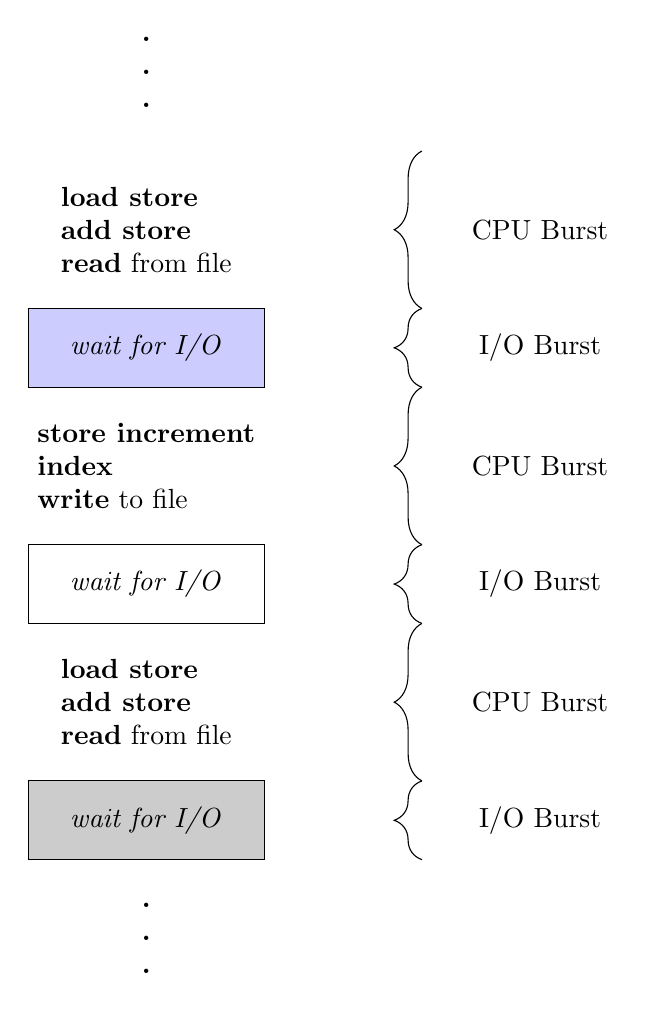
\begin{tikzpicture}
                    \coordinate (io1) at (0,1.5);
                    \coordinate (io2) at (0,4.5);
                    \coordinate (io3) at (0,7.5);

                    \node [align=center] at (0,0) {\textbf{.}\\\textbf{.}\\\textbf{.}};
                    \draw [fill=black!20] (-1.5,1) rectangle (1.5,2);
                    \node at (io1) {\textit{wait for I/O}};
                    \node [align=left] at (0,3) {\textbf{load store}\\\textbf{add store}\\\textbf{read} from file};

                    \draw (-1.5,4) rectangle (1.5,5);
                    \node at (io2) {\textit{wait for I/O}};
                    \node [align=left] at (0,6) {\textbf{store increment}\\\textbf{index}\\\textbf{write} to file};

                    \draw [fill=blue!20] (-1.5,7) rectangle (1.5,8);
                    \node at (io3) {\textit{wait for I/O}};
                    \node [align=left] at (0,9) {\textbf{load store}\\\textbf{add store}\\\textbf{read} from file};

                    \node [align=center] at (0,11) {\textbf{.}\\\textbf{.}\\\textbf{.}};

                    \foreach \y in {1.5,4.5,7.5} {
                        \draw[decorate,decoration={brace,amplitude=10pt},shift={(3,0)}] (0.5,\y-0.5) -- (0.5,\y+0.5);
                        \draw[decorate,decoration={brace,amplitude=10pt},shift={(3,1.5)}] (0.5,\y-1) -- (0.5,\y+1);
                        \node at (5, \y) {I/O Burst};
                        \node at (5, \y+1.5) {CPU Burst};
                    }
                \end{tikzpicture}
                \caption{Alternating Sequence of CPU and I/O Bursts}
            \end{figure}
            \subsubsection{CPU-I/O Burst Cycle}
    \chapter{Deadlocks}
    \chapter{Practicals}
        \section{Introduction to Operating Systems}
        \section{Operating System Structures}
        \section{Processes}
        \section{Threads}
            \subsection{Thread Creation}
            Exercise: Modify sampleThread.c. Create a third thread and this time sum up the first 20 numbers {1,2,...20}.
            Practice passing a struct to the thread:
            \begin{minted}{c}
                typedef struct num_thdata {
                    int thread_no;
                    int sum_to;
                } thsum;
            \end{minted}
                \inputminted{c}{code/threads/prac/sampleThread.c}
            \subsection{Producer and Consumer Threads}
            \subsection{Searching Hash Table Values}
            \subsection{OpenMP}
        \section{Synchronisation}
        \section{Safety Critical Systems}
        \section{Distributed Systems}
        \section{CPU Scheduling}
        \section{Deadlocks}
\end{document}